\documentclass{article}
\usepackage{graphicx} % Required for inserting images
\usepackage{float}
\title{phys 222 class exercises}
\author{Issar Amro}
\date{Fall 2023}

\begin{document}

\maketitle
\section{Lagrange Interpolation}
\subsection{First order Lagrange interpolation.}
\begin{verbatim}
x = np.arange(-25,25, 5)
noise = 1.5*np.random.randint(-10, 10)
y = x**2 + noise
y1 = x**2
plt.scatter(x, y, label = "y = x^2 + noise")
plt.scatter(x, y1, label = "y = x^2")
for i in range(0, len(x)-2):
    x1 = x[i]
    x2 = x[i+1]
    y1 = y[i]
    y2 = y[i+1]
    j = 1 # order
    p = y1 * ((x - x2)/(x1 - x2)) + y2 *((x-x1)/(x2-x1))
    plt.plot(x,p)
plt.ylim(-20, 600)
plt.legend()
plt.show()
\end{verbatim}

\begin{figure}[H]
    \centering
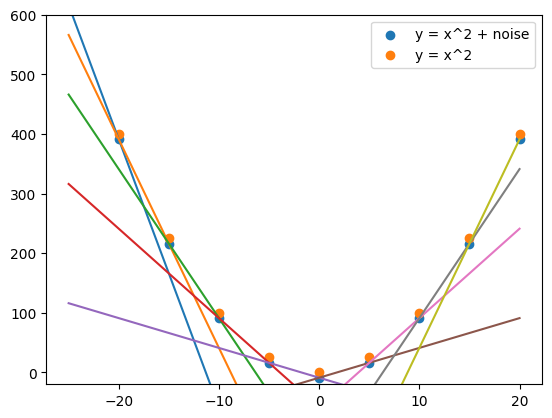
\includegraphics[scale = 0.8]{1stOrderLagrange.png}
\end{figure}
\subsubsection*{notes.}
Each line passes by 2 consecutive data points and the collection of the lines forms an approximation, a bad one, of the function.
\subsection{Second order Lagrange interpolation.}
\begin{verbatim}
x = np.arange(-50,50, 5)
noise = 1.5*np.random.randint(-10, 10)
y = x**2 + noise
y1 = x**2
plt.scatter(x, y, label = "y = x^2 + noise")
plt.scatter(x, y1, label = "y = x^2")
for i in range(0, len(x)-2):
    x1 = x[i]
    x2 = x[i+1]
    x3 = x[i+2]
    y1 = y[i]
    y2 = y[i+1] 
    y3 = y[i+2]
    j = 2 # order
    p = y1 * ((x - x2)/(x1 - x2))*((x-x3)/(x1-x3))
    + y2 *((x-x1)/(x2-x1))*((x-x3)/(x2-x3)) + y3*((x-x2)/(x3-x2))*((x-x1)/(x3-x1))
    plt.plot(x,p)
plt.legend()
plt.show()
\end{verbatim}
\begin{figure}[H]
    \centering
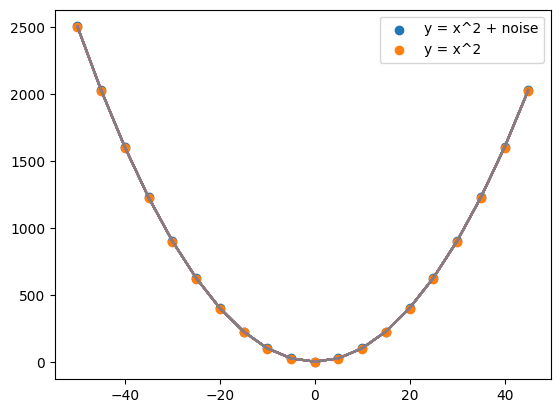
\includegraphics[scale = 0.8]{2ndOrderLagrange.png}
\end{figure}
\subsubsection*{notes} Looping over my data points and using 3 points at a time in the Lagrange polynomials gave me a decent/almost perfect approximation of the function.
\subsection{Defining the order by the number of known data points.}
\begin{verbatim}
x = np.linspace(-100,100, 10)
y = x**2 + 1.5*np.random.randint(-20,20)
y1 = x**2
j = len(x) - 1 # order
for i in np.arange(x[0], x[len(x)-1], 5):
    x_given = i
    y_we_seek = 0
    for i in range(j+1):
        p =1
        for j in range(j+1):
            if j != i:
                p *= ((x_given - x[j])/(x[i] - x[j]))
        y_we_seek += y[i]*p
    plt.scatter(x_given, y_we_seek, color = "r")
plt.scatter(x,y, label = "y = x^2 + noise")
plt.scatter(x,y1, label = "y = x^2")
plt.legend()
plt.show()
\end{verbatim}
\begin{figure}[H]
    \centering
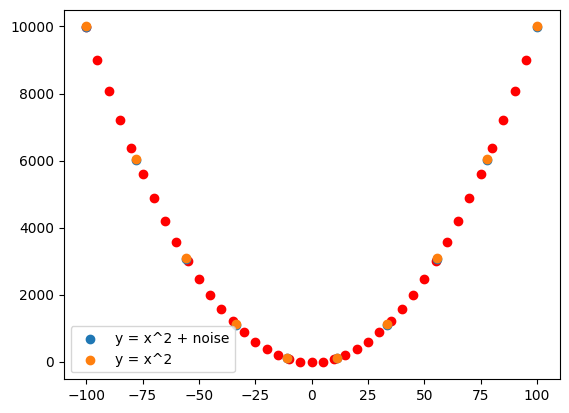
\includegraphics[scale = 0.8]{HighOrderScatter.png}
\end{figure}
\subsubsection*{notes.} I figured here to go to the highest order which is equal to the number of my data points - 1 and fill the points between each 2 consecutive data points.
\subsection{Ploting the function instead of scattered points.}
\begin{verbatim}
x = np.linspace(-100,100, 10)
y = x**2 + 1.5*np.random.randint(-20,20)
y1 = x**2
j = len(x) - 1 # order
x_given_int = []
y_we_seek_int = []
for i in np.arange(x[0], x[len(x)-1], 5):
    x_given = i
    x_given_int.append(x_given)
    y_we_seek = 0
    for i in range(j+1):
        p =1
        for j in range(j+1):
            if j != i:
                p *= ((x_given - x[j])/(x[i] - x[j]))
        y_we_seek += y[i]*p
    y_we_seek_int.append(y_we_seek)
plt.plot(x_given_int, y_we_seek_int, color = "r", label = "the interpolated function")
plt.scatter(x,y, label = "y = x^2 + noise")
plt.scatter(x,y1, label = "y = x^2")
plt.legend()
plt.show()
\end{verbatim}
\begin{figure}[H]
    \centering
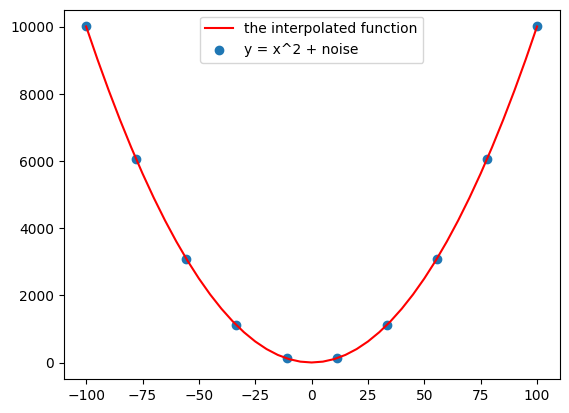
\includegraphics[scale = 0.8]{HighOrderFunc.png}
\end{figure}
\subsubsection*{notes.} Here I stored the "given x" points in an array that represents points between 2 consecutive data points and stored the corresponding "expected y" points that I got from the interpolation and then plotted the function.

\subsection{Trying the above for a linear function.}
\begin{verbatim}
x = np.linspace(-100,100, 10)
y = 3 + x + 0.2*np.random.randint(-20,20)
y1 = 3 + x
j = len(x) - 1 # order
x_given_int = []
y_we_seek_int = []
for i in np.arange(x[0], x[len(x)-1], 5):
    x_given = i
    x_given_int.append(x_given)

    y_we_seek = 0
    for i in range(j+1):
        p =1
        for j in range(j+1):
            if j != i:
                p *= ((x_given - x[j])/(x[i] - x[j]))
        y_we_seek += y[i]*p
    y_we_seek_int.append(y_we_seek)
plt.plot(x_given_int, y_we_seek_int, color = "r", label = "the interpolated function")
plt.scatter(x,y, label = "y = (3 + x) + noise")
plt.scatter(x,y1, label = "y = 3 + x")
plt.legend()
plt.show()
\end{verbatim}
\begin{figure}[H]
    \centering
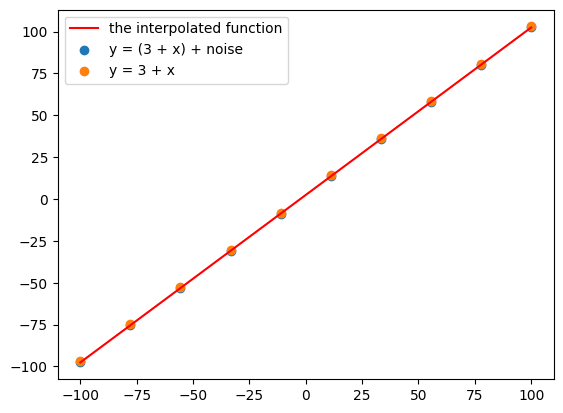
\includegraphics[scale = 0.8]{HighOrderLin.png}
\end{figure}
\subsubsection*{notes.}
I wanted to see if higher orders work also on simple linear functions without causing unwanted oscillations.


\end{document}